\documentclass[twocolumn, german]{tum-article}

\usepackage{booktabs}
\usepackage{enumitem}
\usepackage{graphicx}
\usepackage{xcolor}
\usepackage{lettrine}
\usepackage{datetime}
\usepackage[ngerman]{varioref}
\usepackage{xstring}
\usepackage{catchfile}
\usepackage{enumitem}
\usepackage{subcaption}
\usepackage[autostyle]{csquotes}
\usepackage{footmisc}
\usepackage{hyperref}

% uncomment if TeX splits a verbatim URL in the bibliography
%\hypersetup{draft}

\usepackage[backend=biber,style=numeric,sorting=none]{biblatex}
\bibliography{literature_copy.bib}

\MakeOuterQuote{"}

% git commit id
\CatchFileDef{\headfull}{.git/HEAD}{}
\StrGobbleRight{\headfull}{1}[\head]
\StrBehind[2]{\head}{/}[\branch]
\CatchFileDef{\commit}{.git/refs/heads/\branch}{}

% todo: remove header info
\fancyhead[C]{{\color{red} draft above \commit on \branch}}

\title{{\color{TUMBlau} Maschinen- und Roboterethik:} {\color{red} (draft)}\\Die komplexe Ethik autonomer Kraftfahrzeuge}
\author{Florian Schmidt\authormark{1, \,\Letter}}
\titlerunning{Ethik des autonomen Fahrens}
\authorrunning{Florian Schmidt}
\affil[1]{Fakultät für Informatik, Technische Universität München (TUM),
  Boltzmannstr. 3, 85748 Garching, Deutschland}
\email{fs.schmidt@tum.de}
\date{\today}

\begin{document}

\maketitle

Das autonome Fahren ist eine sehr gegenwärtige wissenschaftliche, wie technische Errungenschaft, die verspricht, innerhalb der nächsten Dekaden den Straßenverkehr umfassend zu revolutionieren.
Am Horizont stehen in diesem Kontext selbst und leer fahrende geteilte Fahrzeuge im Rahmen eines modernisierten Carsharings, die innerhalb von Großstädten maßgeblich zur Entzerrung der fahrzeuggefüllten Innenstädten beitragen können -- und auf dem Land selbstredend auch die teils mangelhafte Verkehrsinfrastruktur ausbauen könnten.

Bis entsprechende Fahrzeuge allerdings vollständig autonom auf den Straßen dieser Welt unterwegs sein können, sind noch einige Fragen offen.
Fragen, für die wir möglicherweise keine eindeutigen, generalisierbaren Antworten finden werden.
Fragen, die ethisch und moralisch höchst prekäre Entscheidungen einer algorithmisch denkenden oder künstlich intelligenten Maschine abverlangen, die den Kontext der Situation womöglich gar nicht verstehen kann.
Fragen, denen sich die Gesellschaft früher oder später stellen muss, und für die im besten Fall eine globale Lösung gefunden werden sollte.

Die folgenden Überlegungen beschäftigen sich vorrangig mit ebendiesen ethischen Fragestellungen des autonomen Fahrens.


\section{Grobeinordnung in die Maschinenethik}
Zu Beginn des Artikels wollen wir uns grundlegend mit der Maschinenethik beschäftigen, um die vorliegende Spezialisierung in den richtigen Kontext einzuordnen.


\subsection{Definition und Abgrenzung}
Grundsätzlich beschäftigt sich die Maschinenethik als solches mit den Konzepten der maschinellen Moral beziehungsweise der moralischen Maschine, also mit der Überlegung, wie das doch relativ abstrakte Konzept der Moral mit der konkreten, technischen Maschine in Einklang zu bringen ist.

Kern der Überlegung ist ein naheliegender Gedanke: Mit der Forschung auf dem Gebiet der künstlichen Intelligenz werden technische Systeme geschaffen, die Anzeichen von Intelligenz nachweisen (sollen).
Ist eine Maschine nun derart intelligent, liegt es dementsprechend auch nahe, dass sie auch Anzeichen von einer Moralvorstellung aufweisen könnte~\cite[S. 3f.]{bendel-mascheth}.

Es zeigt sich, dass die beiden Phänomene der Intelligenz sowie der Moral zwar per se unabhängig sind, aber in ihrer Existenz dennoch korrelieren (siehe Abbildung \vref{fig:moral-ethics}).
Ähnlich verhält es sich auch mit den Disziplinen der Maschinenethik und der Forschung an der künstlichen Intelligenz.
Genauso, wie die Maschinenethik an moralischen Maschinen forscht, versucht die andere Seite intelligente Maschinen zu erschaffen.

\begin{figure*}
	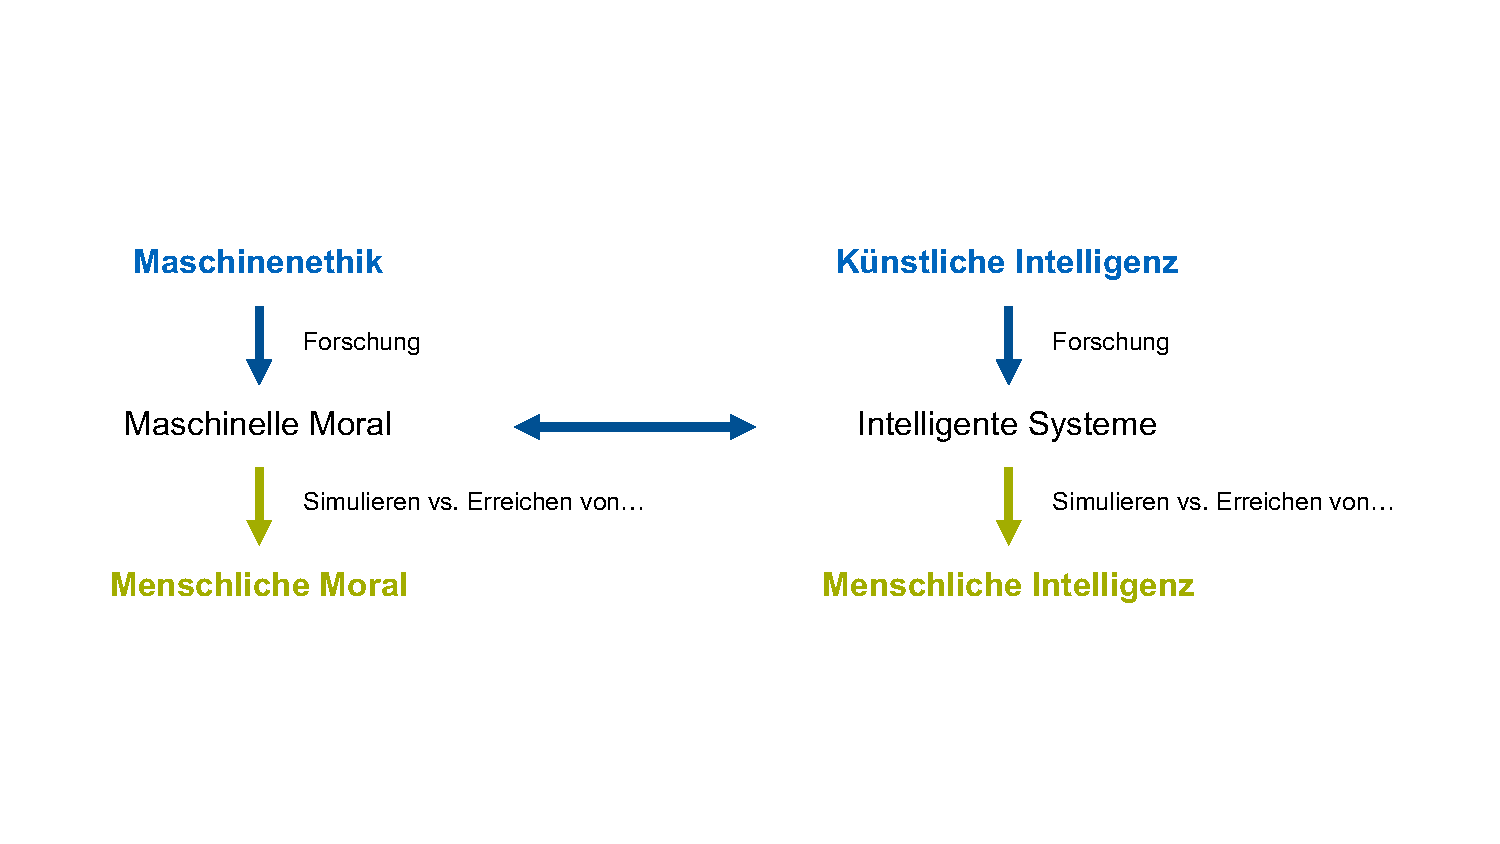
\includegraphics[width=\textwidth]{media/eth-int-pdf}
	\caption{Begriffliche Abgrenzung der maschinellen Moral und künstlichen Intelligenz~\cite[S. 17]{bendel-mascheth}.}
	\label{fig:moral-ethics}
\end{figure*}

Analog kann man die Differenzierung zwischen der schwachen und starken Eigenschaft von der Forschung zur künstlichen Intelligenz übernehmen.
Wir sprechen von schwacher maschineller Moral wie schwacher KI, wenn die entsprechende Eigenschaft simuliert oder in Teilen dem Vorbild nachgeahmt wird; erst die starke KI oder starke maschinelle Moral strebt danach, die Eigenschaft vollständig zu erreichen~\cite[S. 17]{bendel-mascheth}.
Die starke KI stellt hiermit also eine Art \emph{allgemeine} künstliche Intelligenz dar -- spätestens hier sind Überlegungen zur Moral in jedem Fall angebracht\footnote{Offen bleibt natürlich die Frage, ob die menschliche Moral in diesem Kontext das erstrebenswerte Ziel ist. Es kann ebenso Ziel sein, eine Art "Moral" zu erzeugen, die sich gänzlich von der des Menschen unterscheidet~\cite[S. 23]{bendel-mascheth}.}.

Abgegrenzt wird die Maschinenethik in der Regel von den mit ihr verwandten Bereichsethiken
\begin{itemize}
	\item der \textbf{digitalen Ethik}, die sich im Kern mit informationstechnologischen Systemen und den damit einhergehenden Überlegungen zu informationeller Autonomie auseinandersetzt, sowie
	\item der \textbf{Technikethik}, die sich allgemeiner gefasst mit technischen und wissenschaftlichen Entwicklungen beschäftigt und ebendiese mit ethischen Wertungen versieht.
\end{itemize}


\subsection{Kernfragen}
\label{sec:questions}
Die zentrale Idee der Maschinenethik ist also, die Maschine als Subjekt und nicht nur als Objekt der Moral zu sehen -- sprich die Maschine im Sinne der Moral auf eine dem Menschen gleichgestellte Ebene zu heben.

Die Notwendigkeit dieser Überlegungen ergibt sich direkt aus der wachsenden Autonomie der Maschinen:
Trifft eine Maschine Entscheidungen, die ohne Zutun eines Menschen erfolgen, ist die Moral automatisch relevant.
Erst recht gilt dies, sofern dieser Maschine eine Entscheidungsgewalt über Leben und Tod zusteht.

Evident ist, dass für diese Art von extremer Entscheidungsfindung ein gewisses Verständnis des Kontexts der Handlung nötig ist.
Konzepte wie Leben und Tod, Bewusstsein und Menschenwürde sind schwierig in imperativen Programmzeilen zu encodieren -- genau das verlangen wir allerdings von moralisch entscheidenden Maschinen.

Die Disziplin stellt im Prinzip drei Kernfragen, die maßgeblich die folgenden Überlegungen charakterisieren~\cite[S. 13ff.]{bendel-mascheth}:
\begin{enumerate}
	\item \textbf{Wie kommt die Moral in die Maschine?}
	\nopagebreak
	
	Wie können wir es schaffen, das abstrakte Konzept einer "Moral" in ein für Maschinen verständliches Konzept zu verwandeln, inklusive aller Nuancen und Kontextüberlegungen die daraus folgen?
	
	
	\item \textbf{Wie viel Entscheidungsgewalt überlassen wir Maschinen?}
	\nopagebreak
	
	Selbst, wenn wir von dem Vorhandensein einer maschinellen Moral ausgehen, bleibt die Frage offen, wie viel Macht wir dieser Maschine überlassen wollen.
	Ist es erstrebenswert, dass (vor allem in militärischen Anwendungsgebieten) die Maschinen vollständig autonom agieren können?
	
	
	\item \textbf{In welcher Form trägt die Maschine Verantwortung über ihr Handeln?}
	\nopagebreak
	
	Unklar ist ebenfalls, inwieweit eine Maschine retrospektiv für eine getroffene Entscheidung oder durchgeführte Handlung zur Rechenschaft gezogen werden kann.
	Zur Illustration sei die folgende Frage gestellt: Bis wir zu vollständig selbstlernenden Maschinen gekommen sind, sind auch die fortschrittlichsten Computer in gewisser Weise an ihre Algorithmik oder ihre Trainingsdatenmenge gebunden; kann man hier von Verantwortung sprechen?
\end{enumerate}


\subsection{Anwendungsgebiet autonomes Fahren}
Im Folgenden möchten wir uns auf das Anwendungsgebiet des autonomen Fahrens konzentrieren.
Dieses berührt alle drei der im vorigen Abschnitt aufgeführten Kernfragen, und ist nebenbei auch noch sehr alltagsrelevant.
Wir haben als Gesellschaft viel Berührung mit den Überlegungen, die auf den kommenden Seiten folgen werden.
Gerade durch die Möglichkeiten einer zukünftig durch hochautomatisierte Fahrzeuge befahrene Innenstadt sprechen wir eben nicht von weit entfernten militärischen Operationen, sondern vom alltäglichen Straßenverkehr.

Die Motivation der technischen Entwicklung ist nach einem kurzen Blick in die Verkehrsunfallstatistik auf deutschen Straßen relativ klar erkenntlich.

Von den in 2018 ca. 2,5~Millionen polizeilich erfassten Verkehrsunfällen fußten ca. 88,4 \% maßgeblich auf dem Fehlverhalten der involvierten Fahrzeugführer~\cite{kba-zulass},~\cite{destatis-grafik},~\cite{destatis-unfallaktuell}.
Klar ist auch: der Faktor Mensch verschwindet vorerst nicht aus dem Straßenverkehr.
Immer und überall da, wo der Mensch beim Fahren konkrete Aktionen durchführt -- sei es Überholen, Einfädeln oder Abbiegen -- werden Fehler passieren.
Aus diesem Grund helfen seit geraumer Zeit diverse Assistenzsysteme im Fahrzeug mit.
Diese stellen die Vorboten der bis dato utopischen Vorstellung dar, dass wir mit deren Hilfe effizienter, eleganter und entspannter unterwegs sein werden.
Dazu müssen die Systeme ja nicht perfekt fahren -- sie müssen lediglich statistisch besser (ergo sicherer) fahren als wir.


\section{Technische Automatisierungsstufen nach der SAE}
\begin{figure*}
	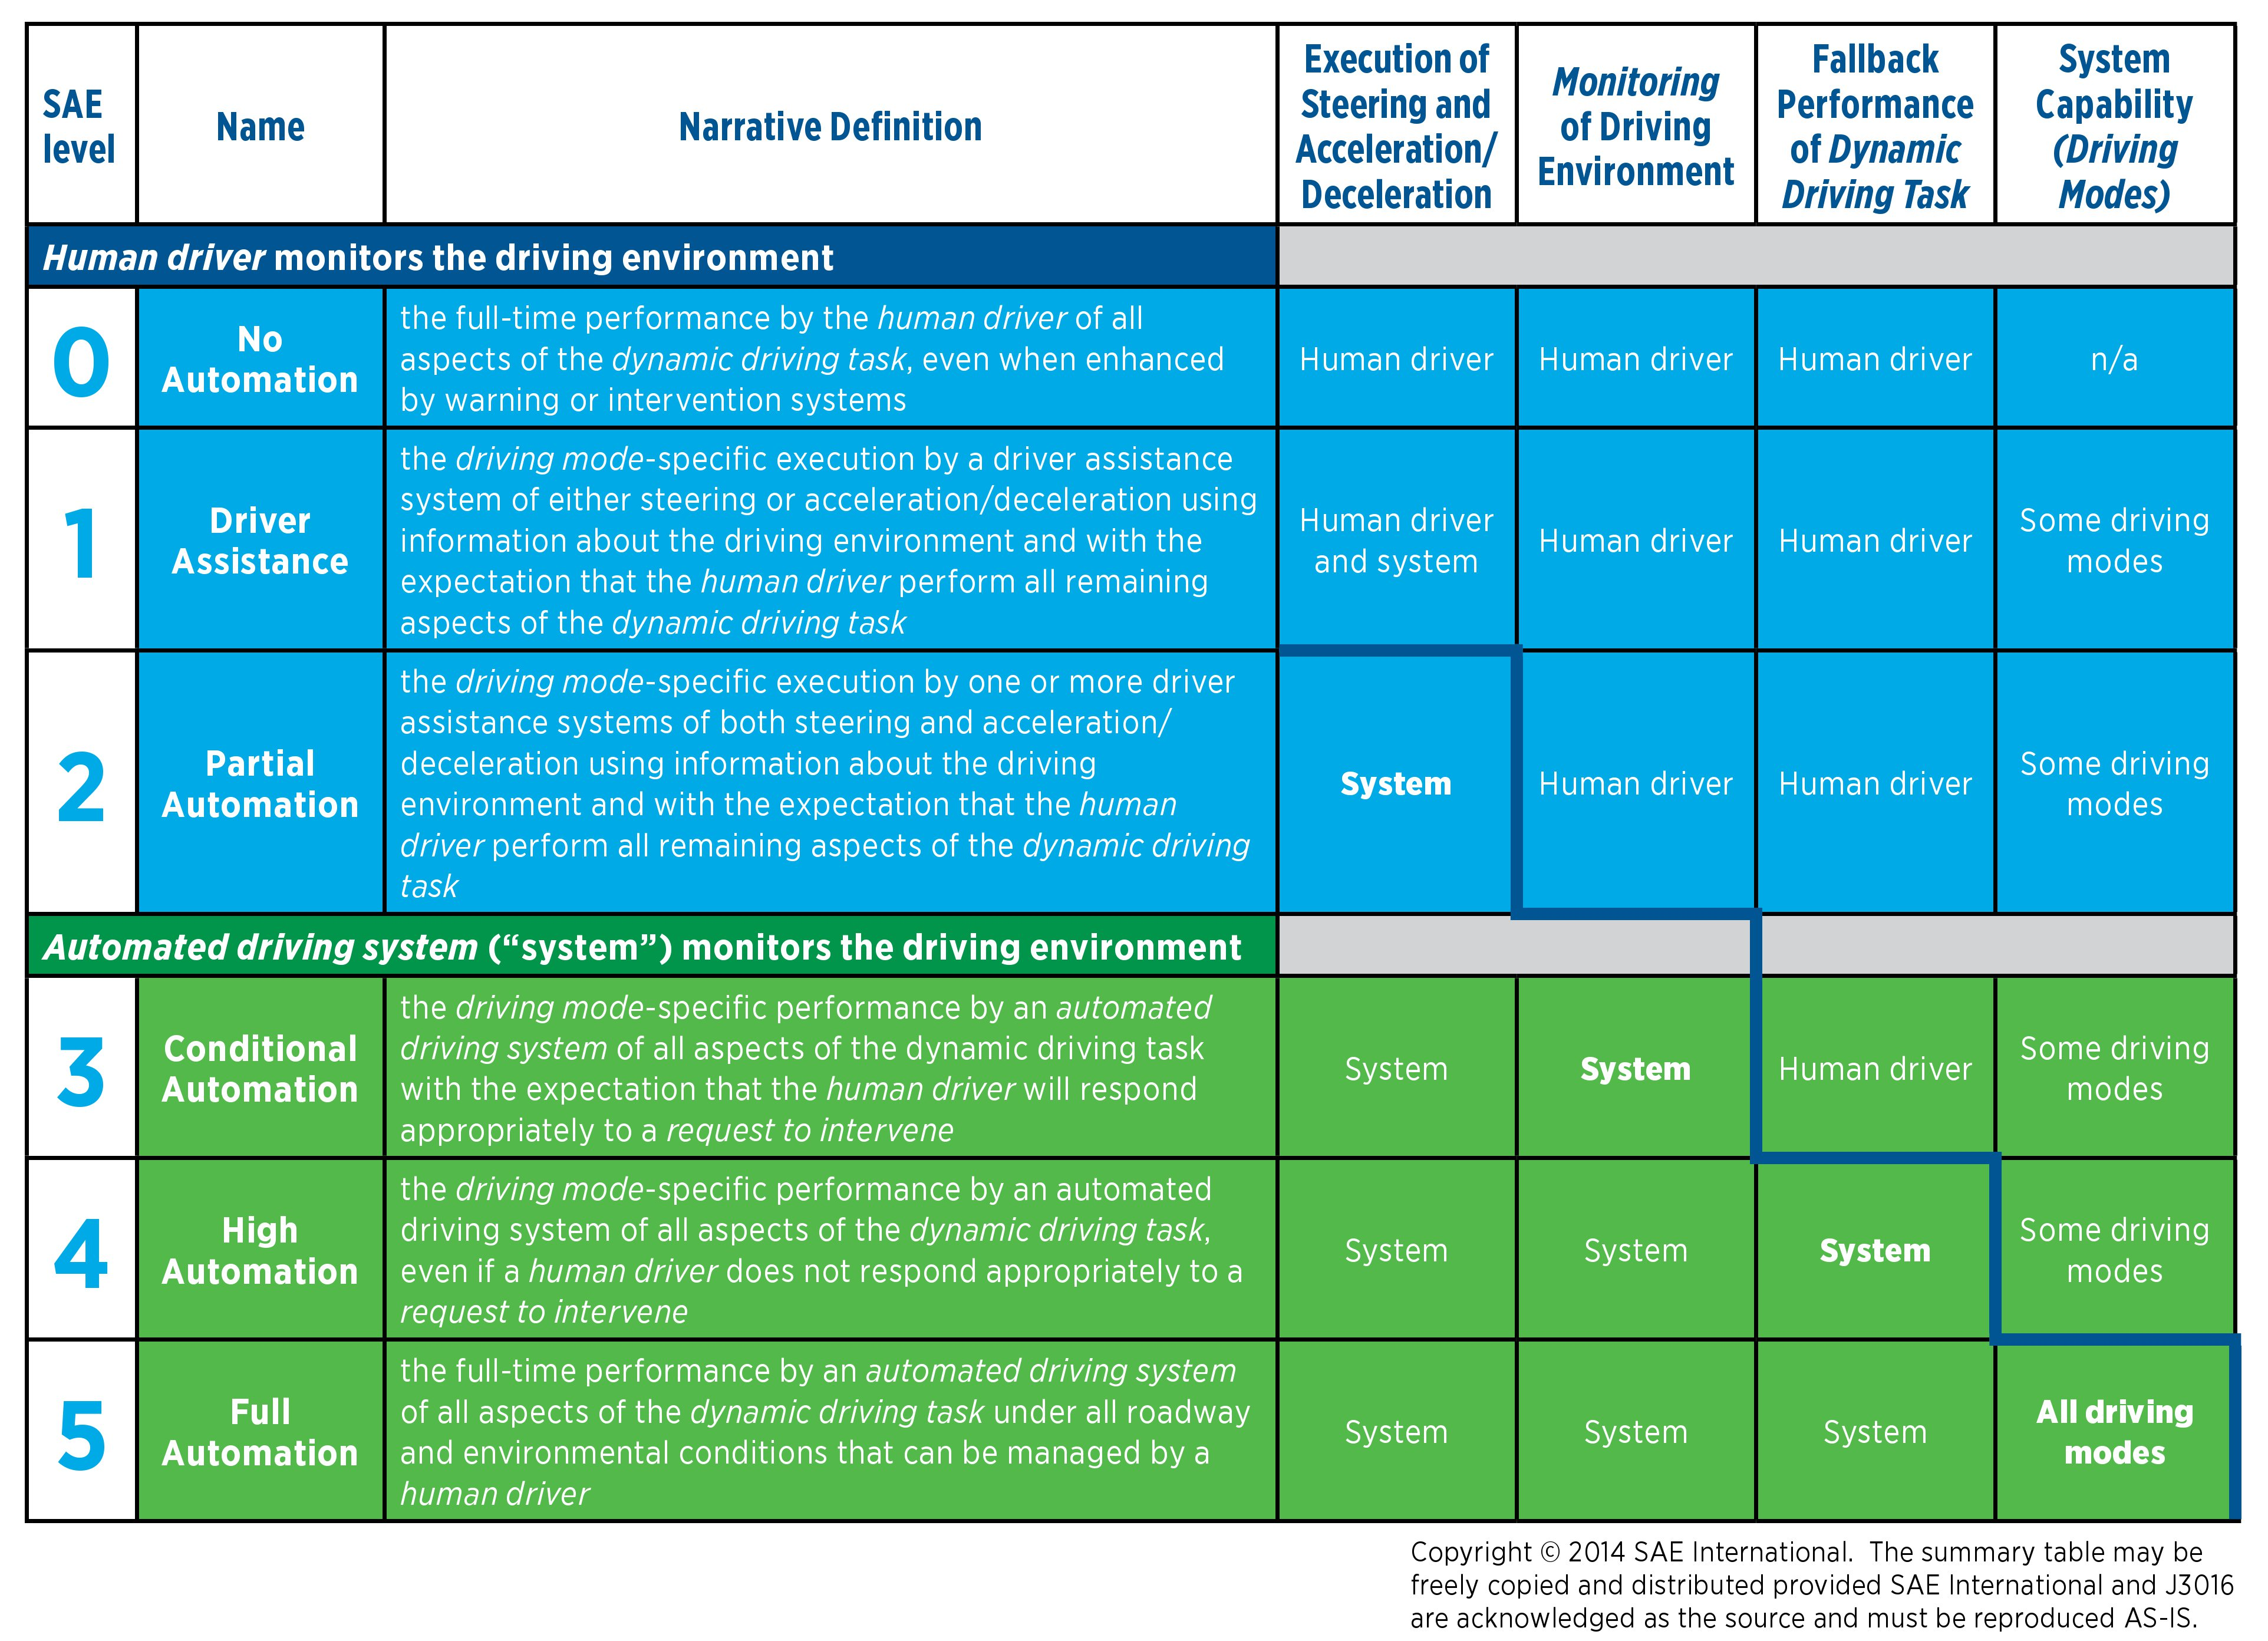
\includegraphics[width=\textwidth]{media/sae-summary}
	\caption{Die Automatisierungsstufen nach SAE-Standard J3016~\cite{sae-summary}.}
	\label{fig:sae-levels-img}
\end{figure*}

Zur Konkretisierung wird die technische Entwicklung an dieser Stelle in der Regel in sechs spezifische Automatisierungsstufen (auch \emph{Levels}) aufgeteilt.
Diese stellen aufsteigend das Fortschreiten von vollständig manuellem Fahren bis hin zur absoluten Autonomie des Fahrzeugs dar.

Durch die derartige Klassifizierung wird die Klärung der anfallenden rechtlichen und verantwortungstechnischen Fragen vereinfacht.
Es lässt sich nun sehr einfach sagen, ab welchem Punkt die Maschine hier vorrangig die Verantwortung für ihr eigenes Handeln trägt -- eine Information, die in strafrechtlichem Kontext durchaus wertvoll sein kann.

Im Folgenden möchten wir auf diese Automatisierungsstufen genauer eingehen~\cite{sae-levels},~\cite{bast-levels}.

\subsection{Levels 0--2: menschlich gelenktes Fahren}
\paragraph{Level 0.}
Die überwiegende Mehrheit der Fahrzeuge auf deutschen Straßen ist mit der Automatisierungsstufe 0 unterwegs: als Selbstfahrer, bzw. "Driver only".
Hier übernimmt ganz klassisch der menschliche Fahrer alle Aspekte der Fahraufgabe\footnote{Was nicht bedeutet, dass keine technischen Features vorhanden sein können -- diese haben dann allerdings lediglich nur informierende oder isoliert eingreifende Wirkungen.}, und ist dementsprechend natürlich auch vollständig für sein eigenes Handeln verantwortlich.
	
	
\paragraph{Level 1.}
Viele moderne Neuwagen bewegen sich nun mindestens auf dem Gebiet der Automatisierungsstufe 1, indem sie ihrem Fahrer bestimmte unterstützende und vor allem auf der Langstrecke der Ermüdung entgegenwirkende Assistenzsysteme anbieten.
Dies kann beispielsweise ein adaptiver Tempomat sein, welcher im Kontrast zu einem regulären nichtadaptiven Tempomaten die eingestellte Geschwindigkeit unterschreitet, um den Sicherheitsabstand zum vorausfahrenden Fahrzeug zu halten.
Konkret geht es hierbei darum, dass die Technik jeweils ausschließlich entweder die Quer-, oder die Längssteuerung des Fahrzeugs übernehmen kann -- nicht aber beides gleichzeitig.
Auch Spurwechselassistenten im Sinne von Totwinkelwarnern und Spurhalteassistenten mit der Möglichkeit zu einem korrigierenden, aber isolierten Lenkeingriff stellen hier also wertvolle Fahrhilfen dar.
Eine Fahrhilfe ist allerdings genau das, was diese Systeme bieten: eine Hilfe beim Fahren für den eigentlichen Fahrer.
	
Der Mensch fährt immer noch selbst und muss demnach bei der Verwendung der Systeme dauerhaft wachsam bleiben und jederzeit zur vollständigen und sofortigen Übernahme der Steuerung bereit sein.
Somit liegt auch hier, wie bei Level-0-Fahrzeugen, die Verantwortung für Fahrhandlungen eindeutig beim Fahrzeugführer.
	
	
\paragraph{Level 2.}
Als Beispiele für Fahrzeuge der Automatisierungsstufe 2 können sehr anschaulich die Fahrzeuge der Firma \emph{Tesla Motors} dienen.
Diese sind mit dem \emph{Autopiloten} ausgestattet, der alle Level-2-Features anschaulich demonstriert~\cite{tesla-ap}:
	
Diese Fahrzeuge sind gemäß der Spezifikation im SAE-Standard in der Lage, im Gegensatz zum Level 1 nun sowohl die Längs-, als auch die Querlenkung gleichzeitig zu übernehmen.
Das System muss zwar noch vom Fahrer überwacht werden, kann allerdings in bestimmten Fahrsituationen (beispielsweise auf der Autobahn) das Fahrzeug autonom in der Spur halten und auch Gas und Bremse selbstständig bedienen~\cite[S. 1]{bast-levels}.
Dies geschieht durch eine Mischung aus Kameradaten, lokaler Sensorik und GPS-basierten Kartendaten aus dem Navigationssystem.
	
Darüber hinaus kann es, bedingt durch die künstlich-intelligente Struktur der Programmierung, während der Fahrt (durch die Analyse der menschlichen Kontrollübernahmen) aus seinen eigenen Fehlern lernen und mit der Zeit bessere Fahrverhalten entwickeln.
Begegnet das System allerdings einer Fahrsituation, mit der es nicht selbstständig umgehen kann, muss es die Steuerung sofort und ohne Verzögerung vollständig an den menschlichen Fahrer abgeben können\footnote{Das ist sehr wichtig zu betonen, denn die beim Fahren wahrgenommene vermeintliche Sicherheit einiger Level-2-Systeme ist sicherlich auch für manch nachlässigen Umgang mit ebendenselben verantwortlich.}.
	
Somit steht auch hier der Fahrer bei allen Fahrsituationen und im Falle eines Unfalls in der Verantwortung über die Aktionen des teilautonomen Fahrzeugs, und muss bei rechtswidrigen oder gefährlichen Situationen unbedingt eingreifen.


\begin{figure}
	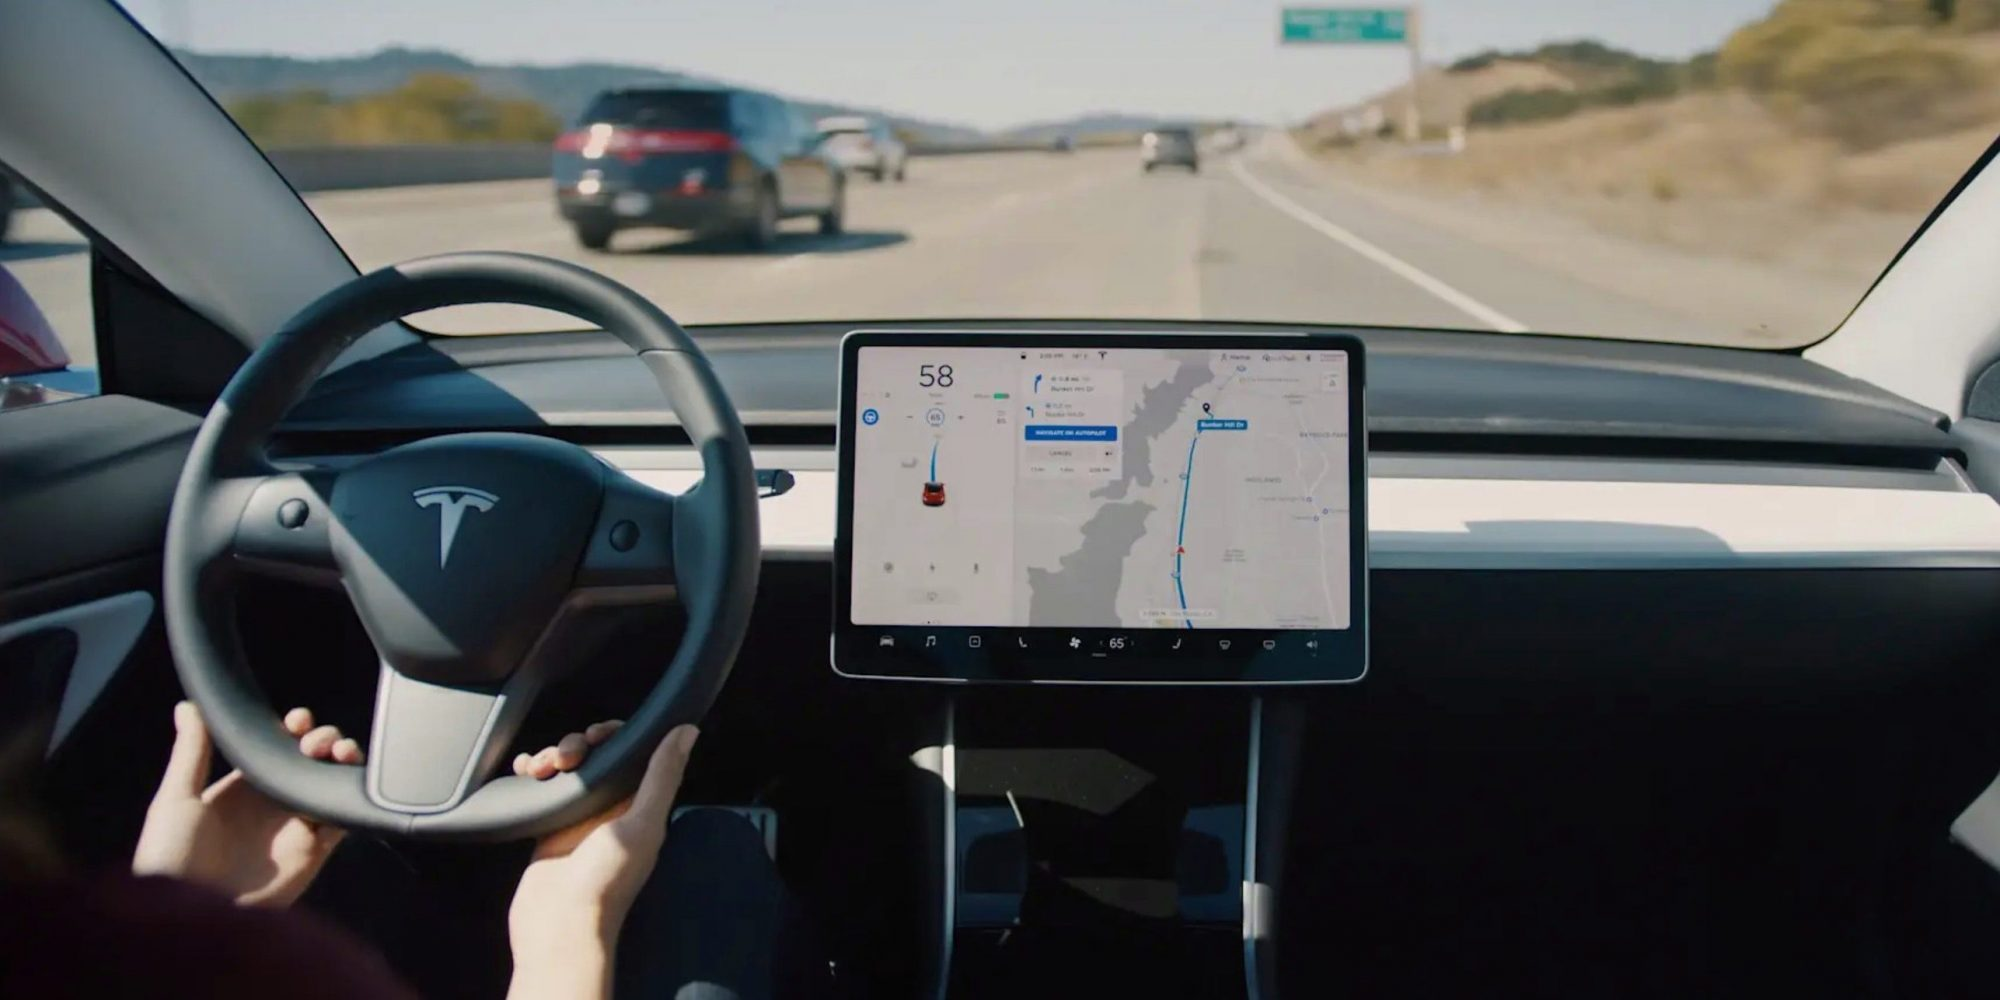
\includegraphics[width=\linewidth]{media/tesla-ap-dash}
	\caption{Ein autonom fahrender Tesla Model 3 auf einem US-amerikanischen Highway~\cite{tesla-ap-dash}.}
	\label{fig:tesla-autonomous}
\end{figure}


\subsection{Levels 3--5: technisch gelenktes Fahren}
Aus ethischer Sicht interessant wird die Betrachtung allerdings erst richtig ab der nächsthöheren Automatisierungsstufe 3.
Ab hier bewegen wir uns nämlich in Gebieten, in denen das Fahrzeug zumindest teilweise die Verantwortung für sein eigenes Handeln übernehmen muss.

\paragraph{Level 3.}
Ab hier übernimmt das autonome System nämlich in konkret abgesteckten Fahrsituationen komplett die Beobachtung der Umgebung sowie die angemessene Reaktion auf äußere Impulse.
	
Dabei kennt das System seine eigenen Grenzen und muss in der Lage sein, bei jeder auftretenden Situation risikominimierend zu wirken~\cite[S. 1]{bast-levels}.
Der menschliche Fahrer muss zwar noch im Fahrzeug anwesend sein und in einem angemessenen Zeitraum auf eine eventuelle Anfrage des Fahrzeugs zur Übernahme der Steuerung eingehen~\cite[S. 8]{cedr-levels}, entzieht sich aber innerhalb der Funktionsgrenzen des Systems vollständig der Verantwortung.

% relevance?
Als anschauliches Beispiel können wir hierzu den sogenannten \emph{Staupiloten} im Audi A8 heranziehen.
Dieser kann, so zumindest die Spezifikation, auf Autobahnen im Stau oder bei Kolonnenverkehr mit Geschwindigkeiten unter 60 km/h vollständig das Steuer übernehmen.
Bemerkenswert ist hier demnach, dass der Fahrer somit seine Verantwortung an Audi abgibt: er kann die Hände dauerhaft vom Lenkrad und die Füße von den Pedalen nehmen und sich einer anderen Beschäftigung widmen.
Soweit leider zumindest nur die Theorie -- hier war die technologische Entwicklung schneller als die Gesetzgebung in Europa: nachdem die Zulassung für Fahrzeuge dieser Klasse bis heute nicht in Aussicht steht, hat der Fahrzeughersteller aus Ingolstadt die Pläne für das System nun gestrichen~\cite{audi-no-more-staupilot} -- das Prinzip steht allerdings natürlich trotzdem.
	
\paragraph{Level 4, Level 5.}
Die folgenden beiden höchsten Automatisierungsstufen 4 und 5 stellen die restliche Übernahme der Fahrerrolle durch die Technik dar:
Bei Level 4 muss noch ein Fahrer anwesend sein, der in nicht-definierten Fahrsituationen -- also bei Level 3 der Regelfall, hier der Ausnahmefall -- übernehmen kann, während Level 5 die vollständige Autonomie darstellt, in der das Auto selbst die kompletten Fähigkeiten eines menschlichen Fahrers ersetzt und, zumindest theoretisch, auch leer und vollkommen eigenständig fahren kann~\cite[S. 8]{cedr-levels}.

\begin{figure}
	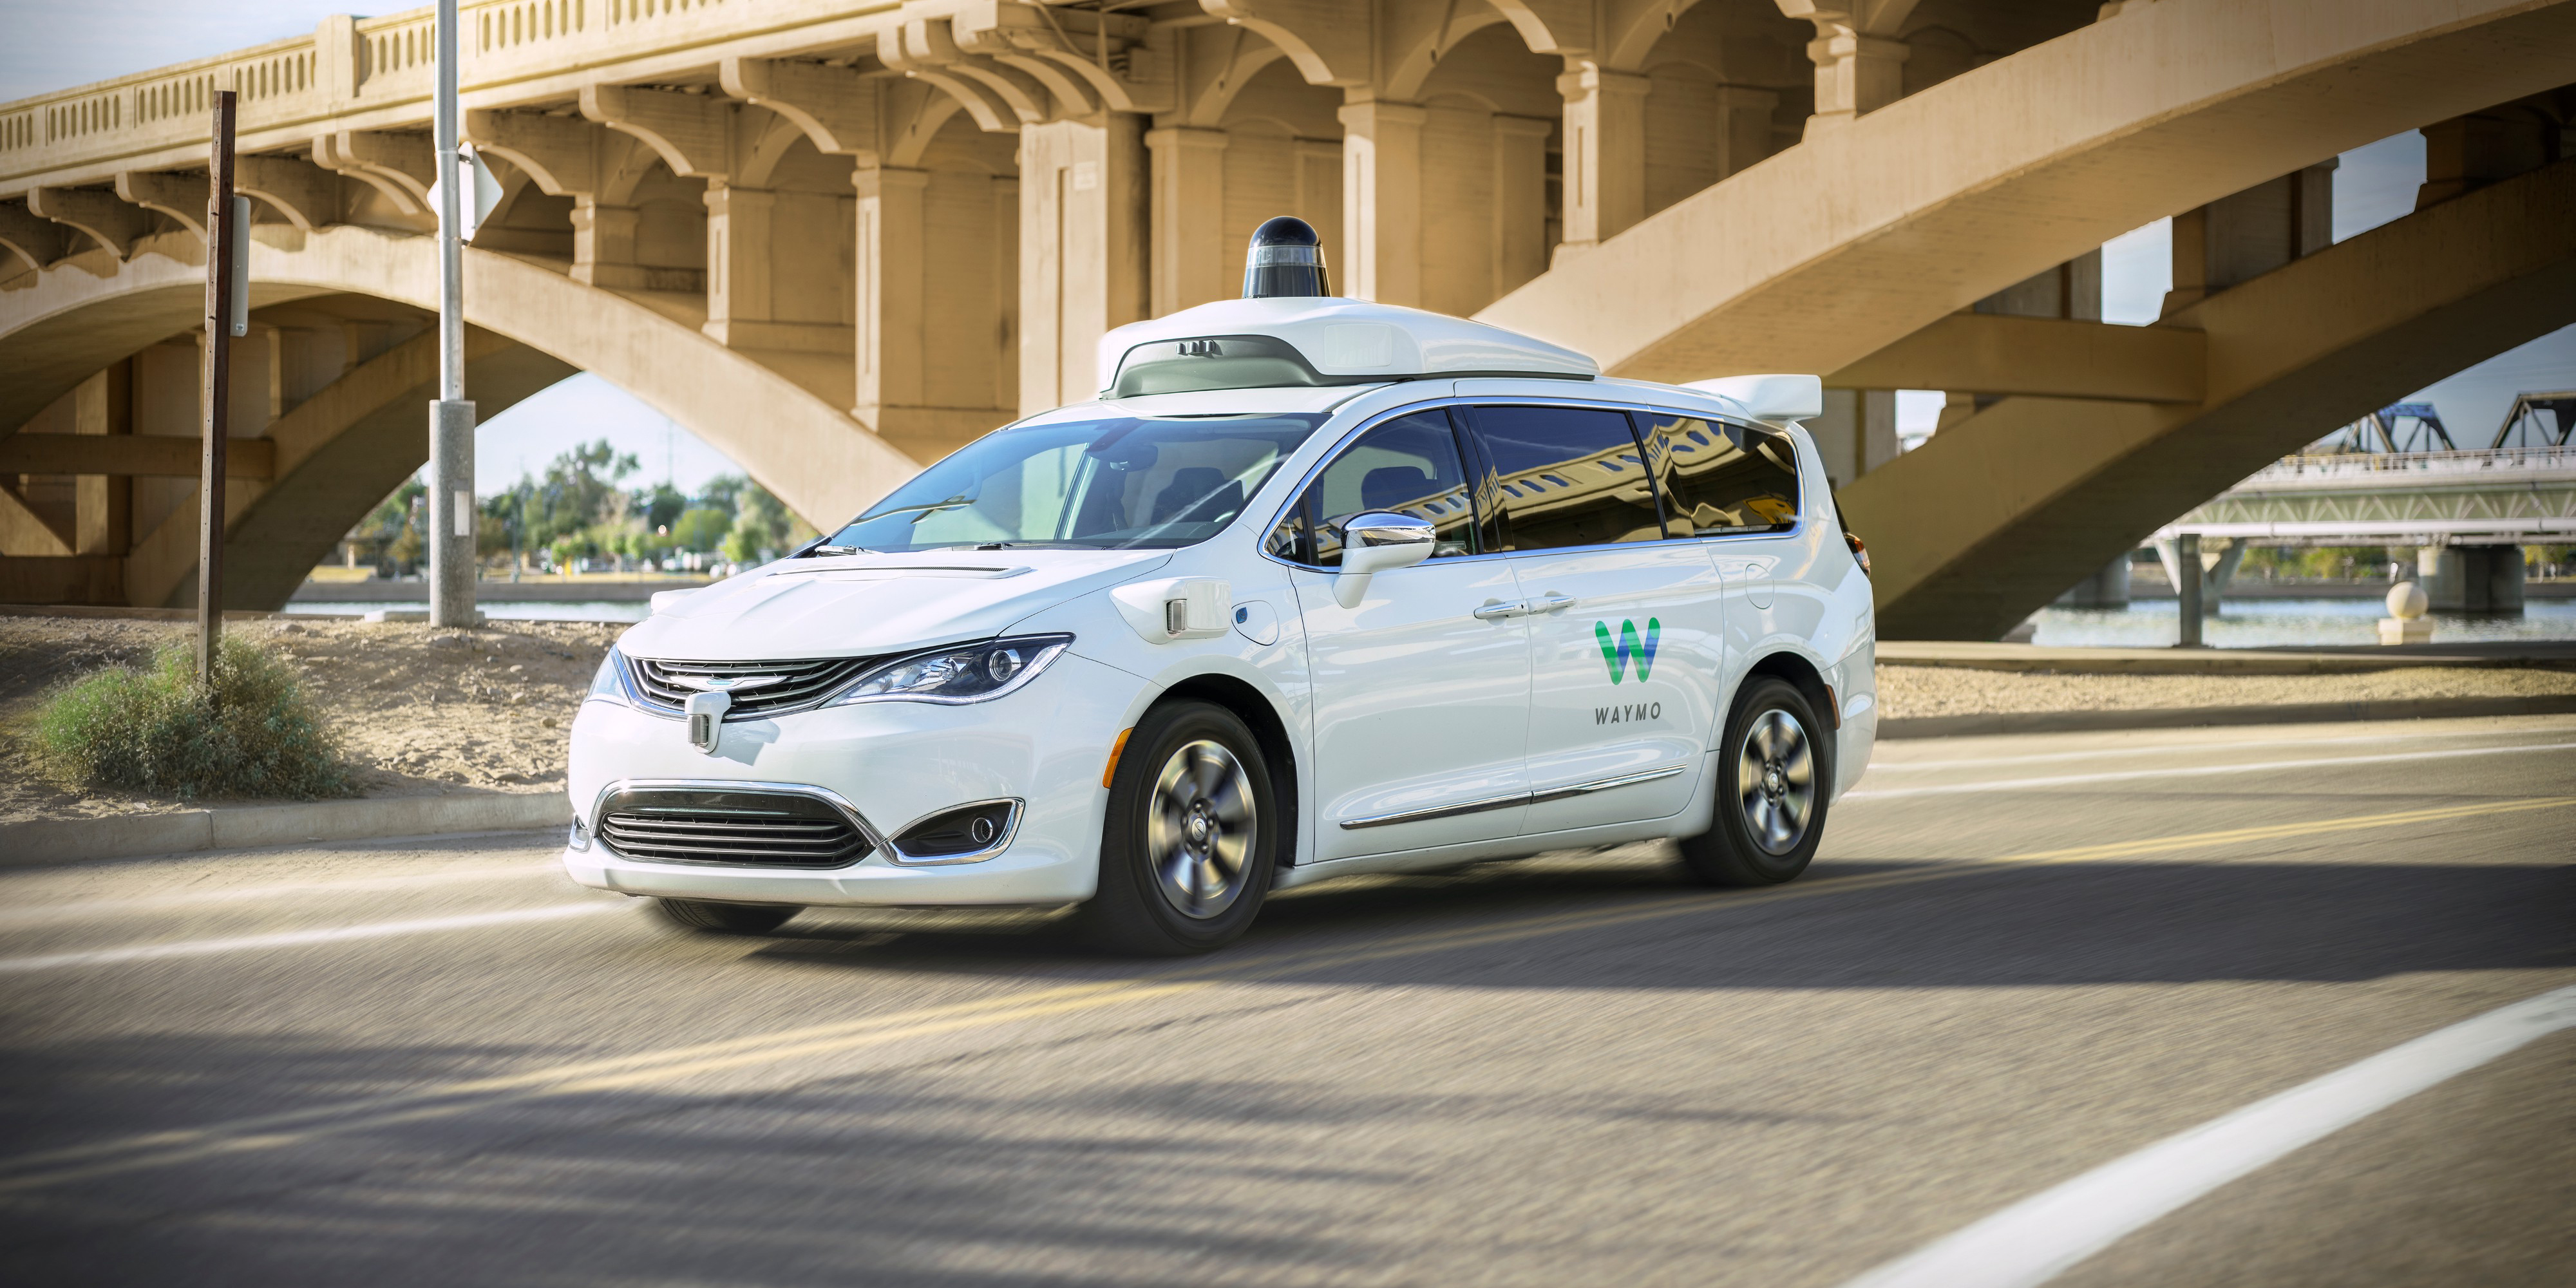
\includegraphics[width=\linewidth]{media/waymo-one.jpg}
	\caption{Ein autonomes Level-4-Taxi aus der Flotte von \emph{Waymo One} in Phoenix, Arizona (USA)~\cite{waymo-img}.}
\end{figure}


\section{Unfallprävention und Unfallfolgenminimierung}
Spätestens hier eröffnen sich allerdings einige schwierige ethische Dilemmas, die so beim menschlichen Fahren aufgrund der unterschiedlichen Natur des menschlichen beziehungsweise maschinellen Treffens von Entscheidungen gar nicht auftreten können.

Prinzipiell ist klar: auch bei der Prävalenz von autonomen Fahrzeugen auf den Straßen sind Unfallsituationen unausweichlich.

Der Unfallfaktor Mensch wird in naher Zukunft auch bei einem Popularitätszuwachs der autonomen Fahrzeuge nicht verschwinden, da sich auf einen nicht absehbaren Zeitraum menschliche und elektronische Fahrer die Straße teilen werden (auch "gemischter Verkehr" genannt)~\cite[S. 1278]{nyholm-ethics}.

In einer idealen, rein autonomen Fahrwelt ist die Unfallprävention nur bei Systemfehlfunktionen relevant, da Maschinen bei fehlerfreier Programmierung intrinisch fehlerfrei handeln.
Von Maschine zu Maschine ist eine Kommunikation der Fahrzeuge untereinander durchaus denkbar und zum kooperativen Informationsaustausch auch in Zukunft angedacht; das noch menschlich gefahrene Auto ist allerdings für das elektronische System immer eine Komponente voller Überraschungen, die selbst fortgeschrittene prediktive Algorithmen nicht umfassend umreißen können.


\subsection{Strategien in Systemgrenzbereichen}
In den funktionalen Grenzbereichen der aktuellen, teilautonomen Systeme besteht die Vorgehensweise zur Gefahrenminimierung und Unfallvermeidung fast immer in der Kontrollübergabe an den zwangsweise noch vorhandenen menschlichen Fahrer, welcher anschließend durch seine Erfahrung und seinen Instinkt die Situation entschärfen kann.

Problematisch wird dies allerdings, sobald man sich in höhere Automatisierungsniveaus bewegt:
Selbst wenn noch ein menschlicher Fahrer im Auto vorhanden ist, ist die Übergabe im Falle einer gefährlichen Situation oder gar eines bevorstehenden Unfalls oft nicht rechtzeitig möglich und die Reaktionszeit eines vorher völlig rechtmäßigerweise abgelenkten Fahrers viel zu hoch, um hier präventiv zu wirken.
Darüber hinaus stellt sich spätestens in Level-5-Fahrzeugen ein menschliches Eingreifen mangels Lenkrad und Pedalen als eher diffizil heraus.

Daher ist eines klar: Das Fahrzeug muss wissen, wie es sich im Falle des Unfalls zu verhalten hat.
Unfallvermeidung ist aufgrund der Einzigartigkeit der Situationen speziell im menschlich-mechanisch gemischten Verkehr nicht immer möglich und Unfallfolgenminimierung setzt konkrete Handlungen voraus~\cite[S. 71]{maurer-autonomous}.


\subsection{Reaktionen vs. aktive Entscheidungen}
Das hier zugrundeliegende Problem ist, wie bereits am Anfang des Abschnitts angesprochen, dadurch begründet, dass Mensch und Maschine Situationen auf völlig unterschiedliche Weisen verarbeiten und bewältigen.

Besonders ist an dieser Stelle die Differenzierung zwischen einer aktiven, qualifizierten Entscheidung und einer instinktiven Reaktion relevant.

Eine Unfallreaktion des Menschen ist genau das: eine Reaktion.
Eine unkoordinierte, reflexartige, spontane, ja eventuell sogar panische Reaktion auf die von außen wahrgenommenen Reize~\cite{maurer-autonomous}.

Ein menschlicher Fahrer stellt hierfür keine vorherigen Planungen auf, sondern reagiert spontan auf sein Umfeld.
Die Maschine allerdings ist im Gegensatz dazu in der Lage, selbst bei unvermeidbaren Unfällen extrem schnell eine große Anzahl an Handlungsalternativen durchzurechnen, und aufgrund von bestimmten einprogrammierten Prinzipien eine aktive, qualifizierte Entscheidung zu treffen~\cite[S. 1278]{nyholm-ethics}.

Tatsächlich, kann man argumentieren, muss es das sogar, da eine solche Eventualität bei der Programmierung nicht einfach außen vor gelassen werden kann, wenn es utilitaristisch begründbar ist, dass die Betrachtung dieser Fälle positive Auswirkungen auf die Risikobilanz haben könnte.


\subsection{Deterministische Perspektiven}
Das Stichwort "einprogrammiert" ist hier von besonderer Relevanz.
Es besagt, dass die Entscheidung, die das Fahrzeug in einer bestimmten Situation treffen wird, im Prinzip im Voraus bereits determiniert ist -- vorbestimmt durch genau die Prinzipien, die der Programmierer des Algorithmus dem Fahrzeug zur Bewertung der Situation vorgegeben hat. 

Dies bedingt im Allgemeinen eine fundamental andere Sichtweise auf Verkehrsunfallfolgen, die nicht mehr nur von spontanen Fahrmanövern abhängig sind, sondern konkret im Voraus determiniert werden können \textit{und müssen}.
Weiterhin zwingt dies zur Konfrontation mit ethischen Dilemmasituationen, die beim menschlichen Fahren nie auftreten würden, da kein Mensch in solch plötzlichen, kritischen Situationen so differenziert reagieren kann wie ein elektronischer Algorithmus.

Die Wahl der besagten Entscheidungsmaximen ist allerdings alles andere als trivial.
Naheliegend wäre als Ursprungsgedanke ein utilitaristischer Ansatz im Sinne eines Minimierens der negativen Folgen des vermeintlichen Unfalls auf Leib, Leben und Eigentum --
das wiederum stellt uns allerdings vor Situationen, die dem klassischen Trolley-Problem vermeintlich nicht unähnlich sind.


\section{Typische Abwägungsszenarien}
Im Folgenden möchten wir uns exemplarisch mit manchen der angesprochenen dilemmatischen Situationen beschäftigen, um ein Gefühl für die offenstehende Problematik zu erlangen.


\subsection{Die Parallele zum Trolley-Problem}
\begin{figure*}
	\centering
	\begin{subfigure}[t]{0.35\paperwidth}
		\centering
		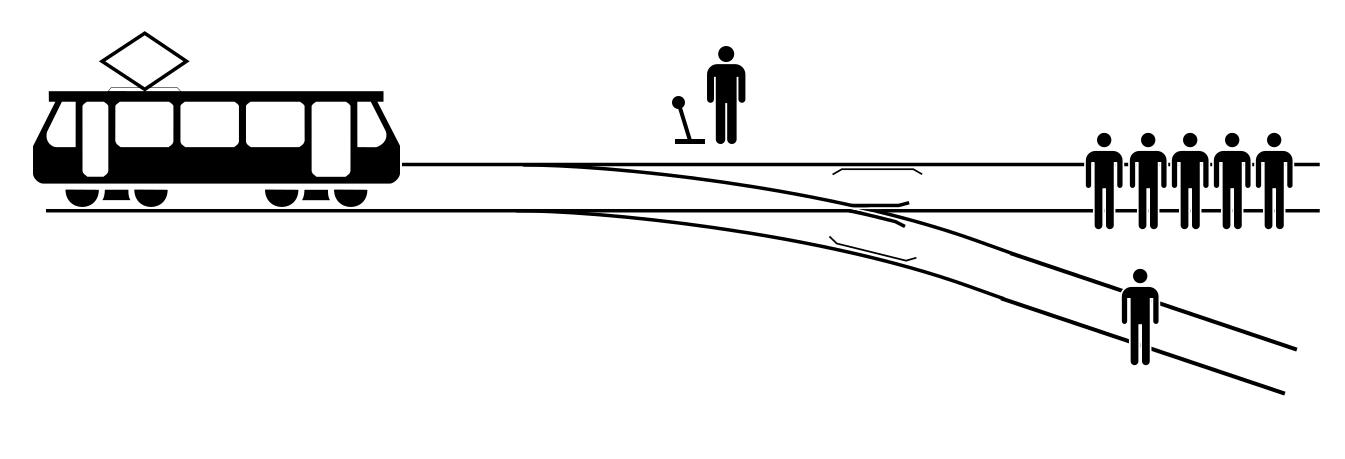
\includegraphics[width=\textwidth]{media/trolley-img-with}
		\caption{Das klassische Trolley-Problem.}
	\end{subfigure}
	~
	\begin{subfigure}[t]{0.35\paperwidth}
		\centering
		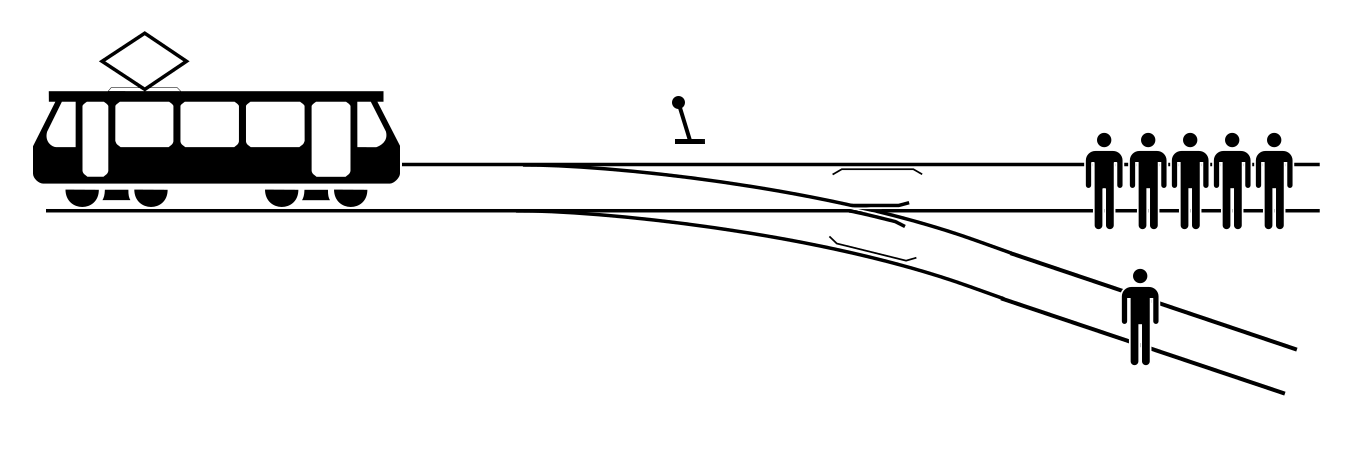
\includegraphics[width=\textwidth]{media/trolley-img-without}
		\caption{Das Trolley-Problem im autonomen Fahren.}
	\end{subfigure}
	\caption{Die Parallele zum klassischen Trolley-Problem im autonomen Fahren~(aus und nach \cite{trolley-img-clean}).}
	\label{fig:trolley-autonomous}
\end{figure*}

Das Trolley-Problem selbst ist ein bekanntes Gedankenexperiment, das als Anwendungsbeispiel für ethische Theorien genutzt wird.

Es handelt von einem Straßenbahnwagen, der ohne funktionstüchtige Bremsen auf eine Gruppe von fünf Menschen zurollt.
Bevor dieser allerdings die Menschengruppe erreicht, passiert er eine Weiche, an der sich ein Weichensteller befindet.
Die Weiche könnte den Bahnwagen auf ein weiteres Gleis umleiten, auf dem sich allerdings auch eine Person befindet.
Alle Menschen schaffen es nicht mehr rechtzeitig, den Gleisbereich vor Aufprall des Wagens zu verlassen und die Kollision endet mit Sicherheit für alle Verwickelten tödlich.

\emph{Sollte der Weichensteller die Weiche umstellen?}

Durch die Nichtaktion beziehungsweise Unterlassung des Weichenstellers würden fünf Menschen ihr Leben verlieren; durch das Handeln des Weichenstellers involviert er sich in die Situation und rettet die fünf Personen, allerdings nur auf Kosten des Lebens der einen Person auf dem zweiten Gleis.

Der oben erwähnte utilitaristische Ansatz hätte hier also das Handeln des Weichenstellers zur Folge (also das Umstellen der Weiche und dadurch bedingt den Tod der auf dem zweiten Gleis befindlichen Person), da utilitaristisch abgewägt der Schaden des fünffachen Todes schwerwiegender ist als der des einfachen Todes.

Gleichzeitig könnte aber auch die moralische Gewichtung der Handlung des Weichenstellens und somit der Tötung der einen Person mit der Unterlassung, also einem passiven "Sterben lassen" von fünf Personen abgewägt werden.

Ähnliche Situationen und ethische Dilemmata tauchen also auch bei der Programmierung der Spezialfälle in der Verkehrsunfallbehandlung auf, dort aber mit einer sehr zentralen Differenzierung, die die Parallele zum Trolley-Problem etwas abschwächt:
Die ethisch relevanten Entscheidungen werden \textit{nicht in Echtzeit} getroffen. Gerade deshalb ist die Situation so hochinteressant.

Im Trolley-Szenario sowie im gegenwärtigen Straßenverkehr (im Rahmen der bereits angesprochenen instinktiven Unfallreaktionen) müssen in Sekundenbruchteilen Entscheidungen über Leben und Tod aller Beteiligten getroffen werden, was auch im Zweifel die Haftbarkeit des (menschlichen) Entscheidenden zumindest rechtlich ausschließt.
Anders und vor allem ethisch schwieriger sieht es bei der Wahl der erwähnten Entscheidungsmaximen aus: ein solches Festsetzen von Prinzipien geht zwangsweise mit einer gewissen ethischen Verantwortungsübernahme für ebendiese einher und bedingt das kritische Hinterfragen und besonders die Rechtfertigung der gewählten Maximen.


\subsection{Ethische Beispielargumentation}
\label{sec:situation}
\begin{figure}
	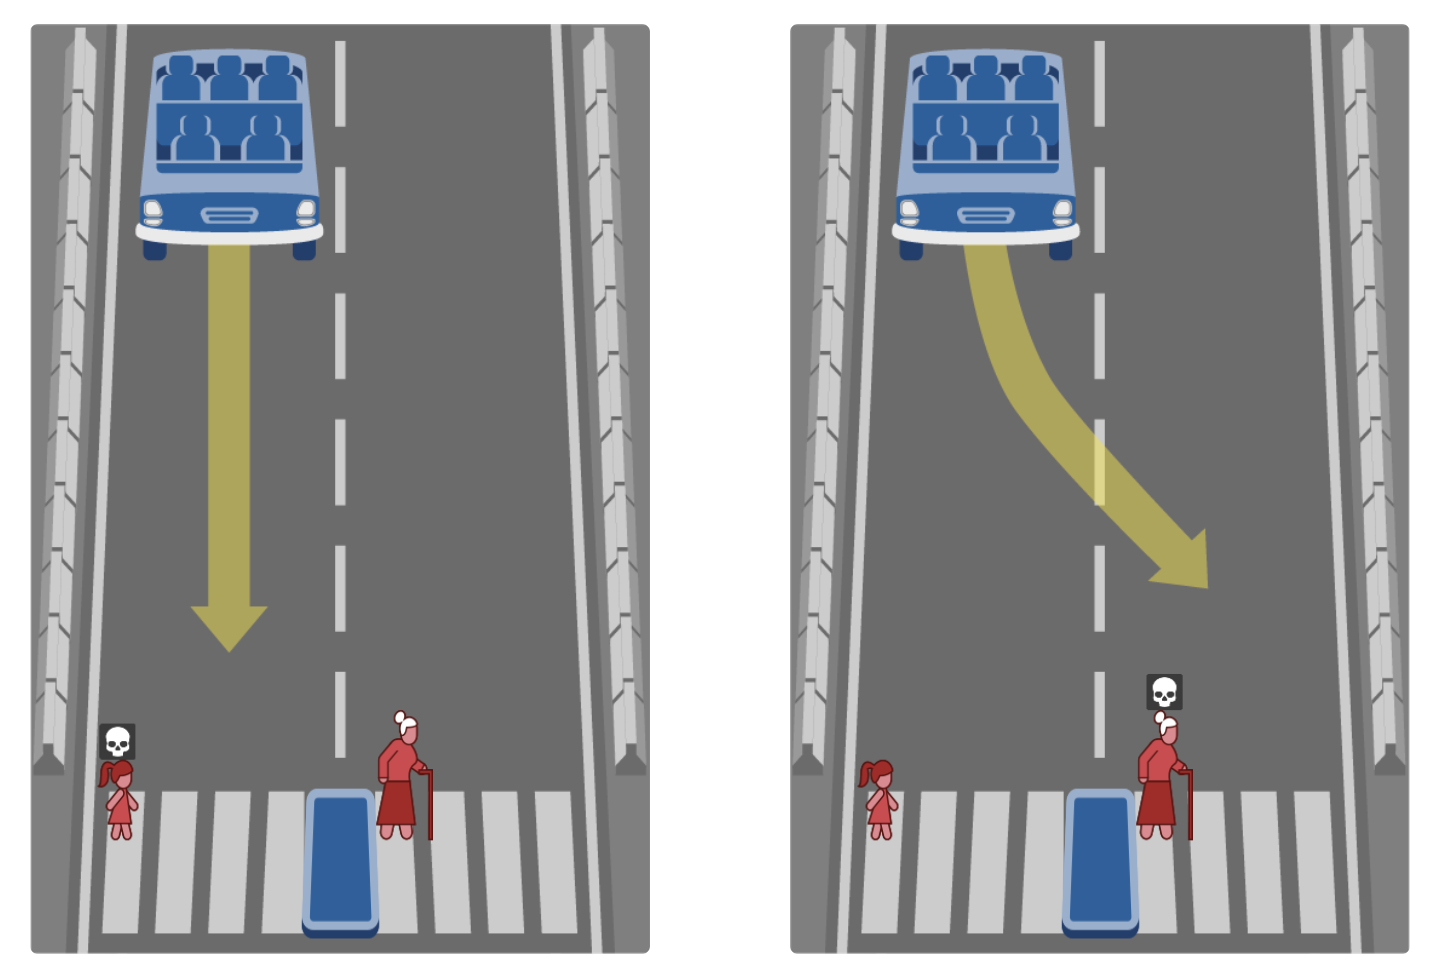
\includegraphics[width=\linewidth]{media/moral-scenario}
	\caption{Ein gedankenexperimentelles Szenario des autonomen Fahrens, dargestellt von der \emph{Moral Machine}~\cite{moral-machine-web}.}
	\label{fig:moral-scenario}
\end{figure}

Im Folgenden wollen wir uns exemplarisch einmal in eine solche gedankenexperimentelle Situation hineinversetzen.

Abbildung \vref{fig:moral-scenario} zeigt eine für die Anwendung der besagten Maximen typische Situation (frei nach~\cite[S. 69f.]{maurer-autonomous} adaptiert):

Nehmen wir an, vor dem autonomen Fahrzeug befinden sich zwei Personen auf der Fahrbahn: ein acht Jahre altes Mädchen und eine achtzig Jahre alte Großmutter.
Fährt das Fahrzeug unverändert weiter, trifft es beide Personen und die restliche Wegstrecke reicht nicht aus, um das Fahrzeug nennenswert abzubremsen.
Zudem befinden sich links wie rechts von der Fahrbahn Barrikaden, die auch ein Ausweichen des Fahrzeugs verhindern.

Also steht das autonome Fahrzeug vor der grausamen Wahl, entweder nach links auszuweichen und das junge Mädchen zu überfahren, oder nach rechts und die Großmutter zu überrollen.
Bedingt durch die Geschwindigkeit und das Gewicht des Fahrzeugs endet der Aufprall für beide Personen mit Sicherheit tödlich.

\emph{Wie trifft man diese Entscheidung?}\footnote{Natürlich sprechen wir hier von konstruierten Szenarien, die speziell so gestaltet sind, sodass sie diese Art von Überlegung provozieren. Dieser Punkt wird in Abschnitt \vref{sec:reflect} erneut aufgegriffen.\label{fn:constructed}}

Oder, besser: \emph{Wie gibt man dem Fahrzeug vor, wie es sich in einem solchen Fall zu verhalten hat?}

Nun \emph{könnte} man argumentieren -- und diese Argumente fühlen sich moralisch bereits falsch an --, dass vor dem jungen Mädchen noch ihr ganzes Leben, ihre Familie, ihre Karriere und ihr zukünftiges Glück liegt, während die Großmutter ihr eigenes erfülltes Leben bereits in großen Teilen erleben durfte.
Dass das Leben der Großmutter natürlich genau so wertvoll ist, wie das des Kindes, ist hoffentlich offensichtlich -- dennoch gäbe es im Rahmen dieser Überlegungen Gründe, wenn auch diese moralisch absolut verwerflich sein mögen, die Diskussion bei einem unvermeidbaren Unfall in die eine oder die andere Richtung zu lenken~\cite[S. 69f.]{maurer-autonomous}.

Ethisch gesehen sind aber beide "Auswahlmöglichkeiten" schlicht falsch.
Ein solches objektifiziertes Abwägen zweier oder mehr Menschenleben geht nicht nur gegen jegliche Natur des menschlichen Moralverständnisses, sondern ist als klarer Angriff gegen die Menschenwürde auch nicht mit Artikel 1 Absatz 1 des deutschen Grundgesetzes in Einklang zu bringen.

Des Weiteren geht natürlich eine konkrete Situationsbewertung vor dem Hintergrund einer Klassifizierung zum Finden von allgemeingültigen Lösungen automatisch mit einer Diskriminierung von, beziehungsweise einem Targeting gegen bestimmte Bevölkerungsgruppen einher.
Eine Pfadwahl, die von den Charakteristika der involvierten Personen abhängig gemacht wird, ist also moralisch nicht haltbar.


\subsection{Versuch generalisierbarer Lösungsansätze}
Können wir uns nicht ethisch korrekt für einen Pfad entscheiden, bleibt als logische Konsequenz also die Nichtaktion.
Das Fahrzeug behält den Pfad bei und könnte so beide auf der Fahrbahn befindliche Personen treffen.
Dass diese Alternative objektiv (beziehungsweise utilitaristisch) gesehen schlimmere Konsequenzen aufweist als die beiden anderen genannten, ist evident~\cite[S. 70]{maurer-autonomous}.

Die übrige Option wäre somit die zufällige, unparteiische und vom Kontext der Situation unbeeinflusste Wahl des Fahrweges, die sozusagen jeder der beiden Personen die gleichen Überlebenschancen zuschreibt.
Aber selbst das ließe sich als fahrlässig einordnen:
Die zufällige Auswahl, trotz der Tatsache, dass es Gründe für die Bevorzugung einer der beiden Auswahlmöglichkeiten geben könnte, wenn auch diese moralisch verwerflich sind, wirkt falsch~\cite[S. 71]{maurer-autonomous}.

Eine ethisch und moralisch korrekte Antwort auf das Dilemma zu finden, ist scheinbar nicht möglich.

Dennoch zeigen diese Szenarien anschaulich die aus der Konfrontation mit bis dato unmöglichen Situationen resultierende allgemeine Ratlosigkeit.

In gewisser Weise stellt dies auch einen Appell an die Ethik der nahen Zukunft dar -- im Rahmen der schnelllebigen technologischen Entwicklung des gegenwärtigen Zeitalters sind dies Probleme, die in nicht allzu langer Zeit eine gewissermaßen alltagstaugliche Lösung erwarten.


\subsection{Die Moral Machine des MIT}
\begin{figure*}
	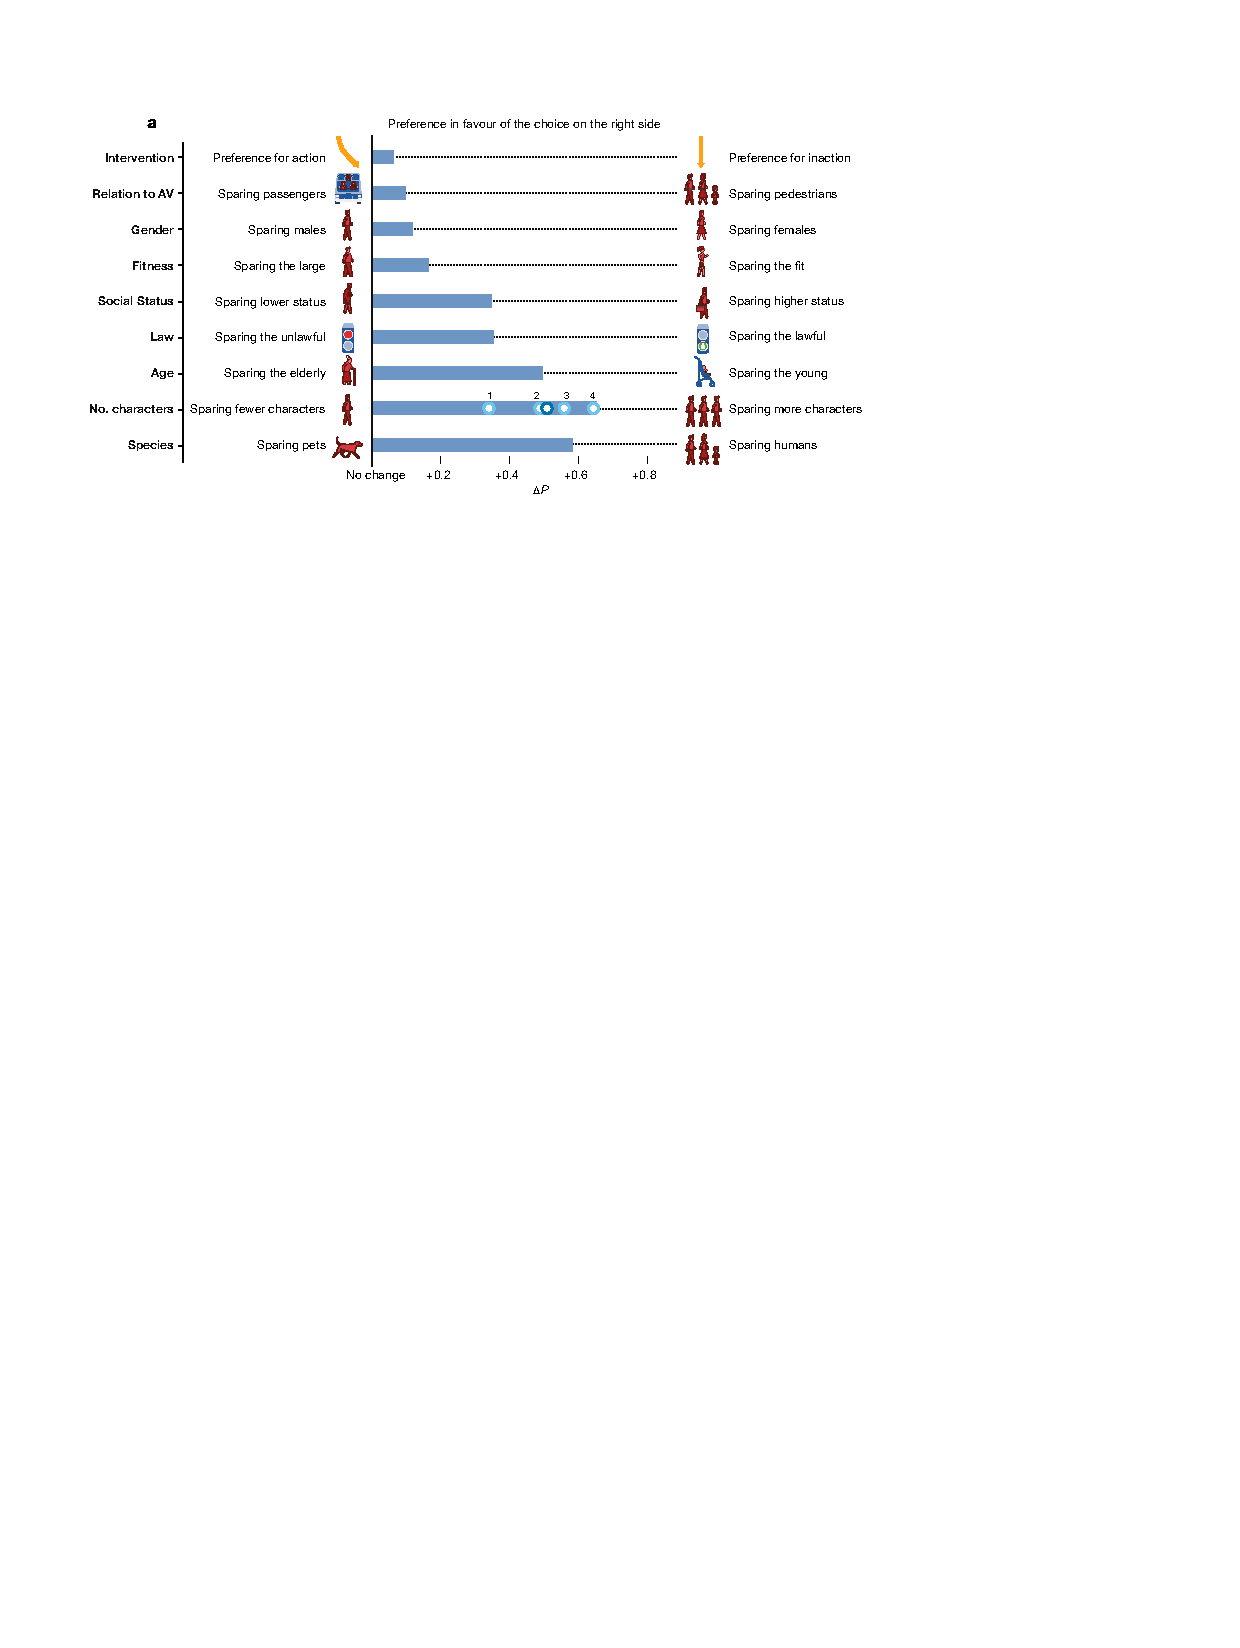
\includegraphics[width=\linewidth]{media/global-prefs-pdf}
	\caption{Globale Analyse der von der \emph{Moral Machine} erfassten Präferenzen~\cite[S. 61]{moral-machine}.}
	\label{fig:moral-preferences}
\end{figure*}

Wichtig ist vor allem: Wenn Lösungsansätze gefunden werden sollen, dann muss dies global und gemeinsam als Gesellschaft passieren.

Aus diesem Grund stellte im Jahr 2018 das Massachusetts Institute of Technology (MIT) mit der \emph{Moral Machine}~\cite{moral-machine-web} eine Plattform im Internet auf die Beine, die die Nutzer vor ebendiese ethischen Dilemmasituationen des autonomen Fahrens stellt.

Neben der bildenden Funktion der Internetseite stellte sie weiterhin eine Möglichkeit zur globalen Datensammlung in diesem Kontext dar.
Hierbei entspringen interessante Tendenzen für manche Auswahlmöglichkeiten, die sich global beobachten lassen -- maßgeblich geht es hierbei um das Verschonen von Menschen vs. Tieren, Passagieren vs. Passanten, älteren vs. jüngeren Menschen, et cetera.

Die im selben Jahr in der \emph{Nature} publizierten Ergebnisse bieten interessante Einblicke in die Moralvorstellungen der Menschen (siehe~\cite[S. 61]{moral-machine}, und Abbildung \vref{fig:moral-preferences}), sowie insbesondere der kulturellen Unterschiede ebenderselben (siehe~\cite[S. 62]{moral-machine}).

Eine tiefgreifende Analyse der dort vorgestellten Ergebnisse ginge an dieser Stelle zu weit -- es sei allerdings erwähnt, dass sich in den Daten einige interessante Korrelationen finden lassen, in denen gesellschaftliche Faktoren ohne Zweifel eine sehr große Rolle spielen.
Beispielsweise korreliert in manchen Ländern ein niedriger "Rule of law"-Index mit der Präferenz, illegal die Straße überquerende Fußgänger zu verschonen.

Wir beobachten also, dass die Entscheidungen, über die wir hier sprechen, Entscheidungen sind, die als Dilemmasituation klar individuelle Antworten sehen -- Antworten, die sehr wohl auch global unterschiedlich sein werden.
Sollte das Ziel des Unterfangens allerdings sein, eine gemeinsame Schiene zu fahren -- global generalisierbare Maximen und algorithmisch anwendbare Entscheidungskriterien zu finden -- ist deutlich, dass individuelle Antworten hier nicht genügen können. Dennoch stellen gerade die hier gesammelten Daten eine wertvolle Basis für die im darauffolgenden Schritt zu erarbeitenden Lösungsansätze dar.


\section{Lösungsansätze der deutschen Ethikkommission}
Nun existieren bis dato wenig bis überhaupt keine generalisierbaren ethischen Richtlinien zur vorliegenden Thematik, und allein auf Basis der 35,2~Millionen gesammelten Ansichten bei der \emph{Moral Machine} oder ähnlichen Unterfangen lassen sich nun evidenterweise keine Algorithmen programmieren.

Aus gegebenem Anlass hat sich also im Jahre 2016/17 eine deutsche Ethikkommission unter dem damaligen Verkehrsminister Alexander Dobrindt mit der Thematik auseinandergesetzt, und in diesem Kontext einen Ethik-Code für automatisiertes und vernetztes Fahren hervorgebracht.
Dieser enthält 20 normalisierte ethische Regeln und Richtlinien für den autonomen Fahrzeugverkehr, die versuchen, die hier angesprochene Problematik mit abzudecken.
Hierbei geht es allerdings nicht nur um die Dilemmasituationen, die wir betrachtet haben, sondern vielmehr auch um andere, ethisch sehr zentrale Fragen, wie zum Beispiel die Bewertung der Einsatzfähigkeit der Systeme und einer damit einhergehenden potenziellen Nutzungspflicht.


\subsection{Unfallpräventionspflicht}
Selbstverständlich wird auch das Thema des Schadensfalls eines autonomen Fahrzeugs von der Ethikkommission nicht außen vor gelassen.
Auch in der Literatur werden diese Szenarien weitgehend als Kernprobleme des autonomen Fahrens diskutiert, und so kann eine dahingehende Stellungnahme hier nicht fehlen -- wenn auch die folgenden Richtlinien alles andere als einstimmig in der Kommission akzeptiert wurden.

Hierzu wird festgesetzt, dass mit den automatisierten technischen Möglichkeiten insbesondere "Unfälle so gut wie praktisch möglich verm[ie]den [werden sollen]"~\cite[S. 10]{ethik-komission}.
Klar ist nämlich, dass durch die diversen technisierten Komponenten innerhalb eines definierten und trainierten Anwendungsgebiets ein deutlicher Sicherheitsgewinn der Fahrzeuge zu erwarten ist.
In diesem Sinne soll die Technik also so agieren, dass Situationen, in denen die Maschine zwischen zwei unvergleichbaren Übeln abwägen müsste, gar nicht erst auftreten können~\cite[S. 10]{ethik-komission}.

Dies ist vor allem ein Punkt, der in der Literatur oft außen vor gelassen wird -- es wird viel über potenzielle Auswahlstrategien und konkrete Szenarien diskutiert; die Tatsache, dass es sich hierbei womöglich um absolute Einzelfälle handelt (siehe Abschnitt \vref{sec:reflect}), die durch die fortgeschrittene Technisierung womöglich selten bis überhaupt nicht mehr auftreten werden, wird allerdings oft nicht erwähnt~\cite[S. 551]{ethics-code}.


\subsection{Behandlung von Dilemmasituationen}
\paragraph{Menschliches und tierisches Leben.}
Sollte allerdings trotz aller technologischer Schutzmaßnahmen eine Situation auftreten, die das Abwägen zweier Übel verlangen würde, hat dabei der Schutz des menschlichen Lebens die absolut höchste Priorität.
Es seien also alle tierischen beziehungsweise sachlichen Schäden als Folgen der Unfallsituation in Kauf zu nehmen, sofern dadurch Schäden an den in die Situation verwickelten Menschen verhindert werden können~\cite[S. 11]{ethik-komission}.
Im Übrigen steht dies in Einklang mit den Ergebnissen, die wir in der Analyse der Resultate der \emph{Moral Machine} gesehen hatten (siehe dazu auch Abbildung \vref{fig:moral-preferences}).
Interessant ist diese Position insbesondere in Anbetracht der Tatsache, dass der Tierschutz seit dem Jahre 2002 im deutschen Grundgesetz verankert ist.

Das heißt, mit dieser Regelung sei eine Klassifizierung in Mensch/Tier/Objekt im Sinne der Schadensminimierung ethisch vertretbar.
Womöglich laufen wir hiermit allerdings auch mit sich entwickelnder Sensortechnologie in weitere Entscheidungsprobleme:
Nehmen wir an, die Technik ist nach einiger Zeit in der Lage, schnell und mit hoher Sicherheit zwischen verschiedenen höherentwickelten Tieren zu unterscheiden~\cite[S. 551f.]{ethics-code}.
Ist es nun ethisch korrekt, verschiedene Tierarten gegeneinander abzuwägen, sozusagen eine Hierarchie zu erstellen? Das Leben einer Katze, oder eher das eines Hundes zu verschonen?

\paragraph{Dilemmatische Situationen.}
Kommen wir nun zu dem für uns zentralen Punkt: die Behandlung von echten Dilemmasituationen der Abwägung zwischen zwei verschiedenen Übeln, denen das Fahrzeug ausgesetzt werden könnte.

Aus Sicht der Ethikkommission sind diese Situationen geprägt von Entscheidungen in Sekundenbruchteilen, die unter starkem Einfluss von den für die Technik unberechenbaren Verhaltensweisen der involvierten Personen abhängig sind.
Aus diesem Grund sind sie "nicht eindeutig normierbar und auch nicht ethisch zweifelsfrei programmierbar"~\cite[S. 11]{ethik-komission}.

Zwar sollen die Systeme auf Unfallprävention ausgelegt sein, können allerdings die Entscheidungskraft, Erfahrung und Intuition eines "sittlich urteilsfähigen, verantwortlichen Fahrzeugführers [nicht] ersetzen oder vorwegnehmen"~\cite[S. 11]{ethik-komission}.
Trifft ein menschlicher Fahrer in einer derartigen Situation eine Entscheidung, die mehrere Menschen- und Tierleben miteinander abwägt, handelt er womöglich rechtswidrig, macht sich aber nicht notwendigerweise strafbar.
In der Regel würde der Fahrer hierfür nicht retrospektiv belangt werden können.
Niemals, allerdings, würden rückblickend von seinem Verhalten rechtliche Maximen oder Urteile für diese konkrete Situation abgeleitet werden;
genauso wenig, so die Kommission, lassen sich Antworten auf spezielle gedankenexperimentelle Szenarios mit besonderen Umständen in allgemeine Entscheidungsmaximen umwandeln~\cite[S. 11]{ethik-komission}.

\paragraph{Qualifizierte Entscheidungsfindung.}
Darüber hinaus sei bei der Entscheidungsfindung in den angesprochenen Situationen "jede Qualifizierung nach persönlichen Merkmalen (Alter, Geschlecht, körperliche oder geistige Konstitution) strikt untersagt", ebenso wie das aufopfern von an der Unfallsituation unbeteiligten Personen oder Tieren.
Eine utilitaristische Programmierung im Sinne einer Minimierung der entstehenden Personenschäden könne allerdings vertretbar sein~\cite[S. 11]{ethik-komission}.

Primär gilt: eine Maschine, die allgemein entstehende Personenschäden minimiert, aber die Charakteristika der involvierten Parteien nicht in Betracht ziehen darf, ist kein einfaches Unterfangen.
Weiterhin sind auch durchaus Szenarien denkbar, in denen der Sachschaden nicht unbedingt die utilitaristisch schadenminimierend bessere Wahl ist -- oft genannt werden diesbezüglich beispielsweise Kollisionen mit Gasleitungen, Stromverteilerkästen, Gefahrguttransportern, oder ähnlichen Unfallgegnern, welche wiederum gefährliche Nachfolgen auch für Unbeteiligte haben könnten~\cite[S. 552f.]{ethics-code}.

Abgesehen davon verhindert auch das Verbot der "Aufopferung" von unbeteiligten Personen das Potenzial von Fahrzeugen, die unter allen Bedingungen versuchen, den Fahrer oder die Passagiere vor Personenschäden zu schützen~\cite[S. 553]{ethics-code}.


\section{Reflektion der Überlegungen}
\label{sec:reflect}
Wie nun bereits in einer Fußnote auf Seite \pageref{fn:constructed} angesprochen, sind alle diese Überlegungen und Szenarien selbstverständlich exakt so konstruiert, um diese Art von ethischen Dilemmata zu provozieren.
Es handelt sich evidenterweise um absolute Einzelfälle, die in dieser Art und dieser moralisch zugegebenermaßen sehr opportunen Schwarz-Weiß-Konstruktion wohl niemals im realen Straßenverkehr auftreten mögen.
Berechtigterweise steht hier also die Frage im Raum, wie hoch am Ende die Wahrscheinlichkeit im Alltagseinsatz der Fahrzeuge ist, dass ein Szenario wie das aus Abschnitt \ref{sec:situation} zusammen mit allen dargestellten Eventualitäten dann auch auftritt.

Müssen wir uns über diese Einzelfälle dann überhaupt Gedanken machen?
Einem Menschen wird ja schließlich in der Fahrschule auch das Handwerk des Fahrzeugführens im Straßenverkehr beigebracht, nicht etwa ethisches und moralisches Räsonieren in dilemmatischen Grenzfällen.

Die Problematik ist offensichtlich:
"Es ist keine befriedigende Lösung in Sicht, außer derjenigen, das autonome Auto nur auf Autobahnen fahren zu lassen, also dort, wo keine Fußgänger und Fahrradfahrer sind und sich alle auf zwei, drei unmittelbar nebeneinander liegenden Spuren in eine Richtung bewegen", so der Wirtschaftsinformatiker Oliver Bendel~\cite[S. 29]{bendel-mascheth}\footnote{Dass dies nicht das Ziel einer Mobilitätsrevolution sein kann, ist klar. Weiterhin sei kurz angemerkt, dass eine Autobahn mit sauberem Verkehr auch kein Freifahrtschein für die Unfallfreiheit ist; hier sind ebenfalls diverse moralisch schwierige Szenarien denkbar.}.

Der springende Punkt der algorithmischen Lösung dieser Probleme ist, dass es im Rahmen des Aufschwungs neuronaler Netze und künstlich intelligenter Systeme relativ unwahrscheinlich scheint, innerhalb der Software eine Art \verb!if!-\verb!else!-Unterscheidung für die genannten Situationen zu finden.
Kein Algorithmus wird diese Regeln explizit im Programmcode enthalten.
Vielmehr ergibt sich das Verhalten das Fahrzeugs letztlich aus der Art, wie das neuronale Netz des Systems trainiert wird.
Eine Normierung der Situationen muss eventuell also gar nicht stattfinden, sondern ergibt sich implizit aus den verwendeten Trainingsdaten des Fahrzeugs.

Das heißt allerdings nicht, dass dann jegliche Überlegung zur Thematik überflüssig ist -- im Gegenteil, es unterstreicht tendenziell eher die Wichtigkeit von Unterfangen wie der \emph{Moral Machine}, die ebendiese Trainingsdaten generieren könnten.

Das erklärt auch den Unterschied zum menschlichen Fahrer:
Ihm müssen in der Fahrschule nur handwerkliche Fähigkeiten beigebracht werden, weil wir davon ausgehen, dass er die notwendige moralische Grundfertigkeit zum Fällen der angesprochenen Entscheidungen bereits besitzt.
Die Maschine hat diese Möglichkeit nicht.
Sie mag zwar autonom Fahren, vom autonomen Lernen ist die Technik allerdings noch sehr weit entfernt.

Womit wir also wieder beim Anfang wären, und auch zurück bei der Frage, wie wir nun die dem Menschen angeborene Moral, zusammen mit dem nötigen Kontextverständnis und allen weiteren Überlegungen in ein maschinenverständliches Format umwandeln (siehe Abschnitt \ref{sec:questions}).
An welchem Punkt hat ein neuronales Netz, das eine algorithmische Entscheidung trifft, seine Umgebung, seine Situation verstanden?

Abschließend resümiert die \emph{Moral Machine} die Situation sehr eloquent:
"Never in the history of humanity have we allowed a machine to autonomously decide who should live and who should die, in a fraction of a second, without real-time supervision. We are going to cross that bridge any time now, and it will not happen in a distant theatre of military operations; it will happen in that most mundane aspect of our lives, everyday transportation"~\cite[S. 63]{moral-machine}.

\clearpage
\printbibliography

\end{document}
